\documentclass[11pt,twoside]{uwthesis}

\usepackage{biblatex}
\usepackage{amssymb,amsmath}
\usepackage{url}
\usepackage{graphicx}
\usepackage{caption}
\usepackage{subcaption}
\usepackage{setspace}
\usepackage{epstopdf}
\usepackage{boxedminipage}
\usepackage{listings}
\usepackage{color}
\definecolor{lightgray}{rgb}{.9,.9,.9}
\definecolor{darkgray}{rgb}{.4,.4,.4}
\definecolor{purple}{rgb}{0.65, 0.12, 0.82}
\lstdefinelanguage{JavaScript}{
  keywords={break, case, catch, continue, debugger, default, delete, do, else, false, finally, for, function, if, in, instanceof, new, null, return, switch, this, throw, true, try, typeof, var, void, while, with},
  morecomment=[l]{//},
  morecomment=[s]{/*}{*/},
  morestring=[b]',
  morestring=[b]",
  ndkeywords={class, export, boolean, throw, implements, import, this},
  keywordstyle=\color{blue}\bfseries,
  ndkeywordstyle=\color{darkgray}\bfseries,
  identifierstyle=\color{black},
  commentstyle=\color{purple}\ttfamily,
  stringstyle=\color{red}\ttfamily,
  sensitive=true
}

\lstset{
   language=JavaScript,
   backgroundcolor=\color{lightgray},
   extendedchars=true,
   basicstyle=\footnotesize\ttfamily,
   showstringspaces=false,
   showspaces=false,
   numbers=left,
   numberstyle=\footnotesize,
   numbersep=9pt,
   tabsize=2,
   breaklines=true,
   showtabs=false,
   captionpos=b
}

\usepackage[unicode=true,
            colorlinks=true,
            linkcolor=blue]{hyperref}


\bibliography{refs}


\begin{document}

% preliminary pages
%
\prelimpages
%
% ----- copyright and title pages
%
\Title{Carbon.js: A Modern Toolkit for Building Web Applications for Systems Biology}
\Author{Stanley Gu}
\Year{2014}
\Program{UW Bioengineering}

\Chair{Herbert M. Sauro}{Associate Professor}{Department of Bioengineering}
\Signature{James B. Bassingthwaighte}
\Signature{Daniel L. Cook}
\Signature{Thomas Hazlet}
\Signature{Rick James}

\copyrightpage

% \titlepage  

% --- sample stuff only -----
% unusual footnote not found in a real thesis
% You just use the \titlepage as commented out above

{\Degreetext{General Examination \\
  submitted in partial fulfillment of the\\ requirements for the degree of}
 \def\thefootnote{\fnsymbol{footnote}}
 \let\footnoterule\relax
 \titlepage
 }
\setcounter{footnote}{0}

% --- end-of-sample-stuff ---
 
%
% ----- signature and quoteslip are gone
%

%
% ----- abstract
%


\setcounter{page}{-1}
\abstract{%

This sample dissertation is an aid to students who are attempting
to format their theses with \LaTeX, a sophisticated
text formatter widely available at the University of Washington
and other institutions of higher learning.
 
\begin{itemize}
\item It describes the use of a specialized
macro package developed specifically for thesis production
at the University.
The macros customize \LaTeX\ for the correct thesis style,
allowing the student to concentrate on the substance of
his or her text.%
\footnote{See Appendix A to obtain the source to this
 thesis and the style file.}
\item It demonstrates the solutions to a variety of
formatting challenges found in thesis production.
\item It serves as a template for a real dissertation.
\end{itemize}
}
 
%
% ----- contents & etc.
%
\tableofcontents
\listoffigures
%\listoftables  % I have no tables
 
%
% ----- glossary 
%
\chapter*{Glossary}      % starred form omits the `chapter x'
\addcontentsline{toc}{chapter}{Glossary}
\thispagestyle{plain}
%
\begin{glossary}
\item[Angular.js]
\item[Canvas]
\item[D3.js]
\item[DOM] 
\item[AJAX]
\item[HTML]
\item[HTML5]
\item[SVG]

\end{glossary}
 
%
% ----- acknowledgments
%
\acknowledgments{% \vskip2pc
  % {\narrower\noindent
  The author wishes to express sincere appreciation to the
  University of Washington and the Department of Bioengineering.
  % \par}
}

%
% ----- dedication
%
\dedication{\begin{center}

%to my dear wife, Joanna

\end{center}}


% text pages
%
\textpages
\chapter{Introduction}

\section{Motivation}

Computational Systems Biology is a growing inter-discplinary field that focuses on understanding complex biological systems. \autocite{kitano2002computational}
Traditionally, biologists would build scientific hypotheses on paper and then test them through \textit{in vitro} and \textit{in vivo} experimentation, now this work is assisted by computer software.
Systems biology is the progression of classical molecular biology from a qualitative to a quantitative science.
Software can help not only data collection and analysis, but formulate and test hypotheses through virtual experimentation.
Computational models described here are formal descriptions of a biomedical process, and in particular intracellular kinetic models described by ordinary differential equations.
A simulation is a dynamic realization of the model that describes the evolution of the process from a particular set of starting conditions, which may be tested experimentally.
Simulation experiments allow research in areas that were once difficult to approach by providing information that is difficult or impossible to measure. \autocite{edwards2001silico}
Thus, progress in Systems Biology can result in accelerated drug discovery, safer medicines, and improved understanding of pathogenesis. \autocite{kitano2010grand, mack2004can}

In other research-oriented industries where software and simulation has been integrated, such as automobile, aerospace, and telecommunication, have seen immense cost savings and increases in efficiency.
Virtual cars are "driven" and virtual aircrafts "flown" under simulated conditions before production and manufacture. \autocite{ghosh2010connecting}
Evidence suggests that the Systems Biology software and modeling tools still has some more room to grow in order to realize its full potential (for example, the pharmaceutical industry spends 25\% of revenues on research and development, almost twice that of any other R\&D industry). \autocite{economist2005models}

So what are the challenges in modeling?
It may be a difficult task for some researchers to write models, as they are usually phrased in terms of differential or stochastic equations.
Once completed, models may be so far removed from the biological context that is hard to identify what the model is about or what assumptions were made.
Thus, these models are difficult to search for by a computer and are not readily accessible to the community.
Simulations have generated a large amount of data.
However, when the underlying simulation procedure and model are not available, these results are difficult to interpret.

The Systems Biology community is actively addressing these concerns through the development of standards.
The range of standards include the description of computational models \autocite{hucka:2002d, LloydCellML2004}, annotation of the model assumptions and constituents \autocite{novere2005minimum}, annotation of simulation experiments \autocite{kohn2008sed}, and annotation of simulation data \autocite{dada2010sbrml}.
However, these model standards and ontologies are abstract and meant primarily to be understood by computer scientists and software developers.
It is the role of software applications to help mitigate this kind of complexity.
A modeler should not have to be concerned with all these technical details and be allowed to focus on creating and analyzing the model.

Thus, it is the goal of this work to increase researcher productivity by bridge the gap between modeling standards and end users.

\subsection{Why the Web?}

The bulk of the work described in this writing is centered around the web browser as the primary user interface, so it is worth discussing why the web was chosen as the target platform.
Due to not having any experience with graphical software development at the start of this dissertation project, this author surveyed the various software platforms available to invest in.
In order to make an application widely available to researchers, writing cross platform applications is a technical challenge, especially for research groups with limited software engineering resources. \autocite{cusumano1999netscape}
Cisco estimates that the number of devices connected to the Internet will swell from about 10 billion today to 50 billion by 2020 \autocite{clark2014internet}
With the advent of modern browsers, HTML5 based web applications are cross-platform, off-line capable, and perpetually updated. \autocite{o2007web}

By virtue of expecting users to have a network connection, web applications may also be more social.
A recent study \autocite{dabbish2012social} suggests that social networks can increase productivity.
Dabbish et al. surveyed users of the open software repository GitHub, and found that transparency and collaboration through a web interface promotes user innovation, knowledge sharing, and community building.

Scientific web applications may also change the way models and results are made available to the scientific community.
Models are often discovered through journal publications, which contain a text description of the model, static tables and charts of the results, and possibly a supplementary section with data and the encoded model description file in standard format (such as SBML or CellML).
With the rise of online journals, the viewing application is often the web browser.
The tools developed in this dissertation can allow the model and reproducible simulation results directly embedded or linked into an interactive figure in the article itself.

\section{Specific Results}
\subsection{Aim 1 - Chapter~\ref{chap:graphene}: Produce a web library for building interactive and graphical applications}
\subsection{Aim 2 - Chapters~\ref{chap:tidal},~\ref{chap:redox}: Integrate Graphene into new and existing applications}
\subsection{Aim 3 - Chapters~\ref{chap:carbon},~\ref{chap:engine}: Build server-side architecture for modeling applications}


\newcommand{\bgamma}{\mbox{\boldmath $\Gamma$}}

\newcommand{\bL}{\mbox{\boldmath $L$}}

\newcommand{\bT}{\mbox{\boldmath $T$}}

\newcommand{\bI}{\mbox{\boldmath $I$}}

\newcommand{\bM}{\mbox{\boldmath $M$}}

\newcommand{\bm}{\mbox{\boldmath $m$}}

\newcommand{\bN}{\mbox{\boldmath $N$}}

\newcommand{\bE}{\mbox{\boldmath $E$}}

\newcommand{\bA}{\mbox{\boldmath $A$}}

\newcommand{\bB}{\mbox{\boldmath $B$}}

\newcommand{\bK}{\mbox{\boldmath $K$}}

\newcommand{\bP}{\mbox{\boldmath $P$}}

\newcommand{\bx}{\mbox{\boldmath $x$}}

\newcommand{\bU}{\mbox{\boldmath $U$}}

\newcommand{\bV}{\mbox{\boldmath $V$}}

\newcommand{\bZero}{\mbox{\boldmath $0$}}

\newcommand{\bLo}{\mbox{\boldmath $L_0$}}

\newcommand{\bNo}{\mbox{\boldmath $N_0$}}

\newcommand{\bNr}{\mbox{\boldmath $N_R$}}

\newcommand{\bSi}{\mbox{\boldmath $S_i$}}

\newcommand{\bSd}{\mbox{\boldmath $S_d$}}

\newcommand{\bdSi}{\mbox{\boldmath $dS_i$}}

\newcommand{\bdSd}{\mbox{\boldmath $dS_d$}}

\newcommand{\bS}{\mbox{\boldmath $S$}}

\newcommand{\bdS}{\mbox{\boldmath $dS$}}

\newcommand{\bdt}{\mbox{\boldmath $dt$}}

\newcommand{\bdSdt}{\mbox{$\displaystyle \frac{\bdS}{\bdt}$}}

\newcommand{\bdSddt}{\mbox{$\displaystyle \frac{\bdS_d}{\bdt}$}}

\newcommand{\bdSidt}{\mbox{$\displaystyle \frac{\bdS_i}{\bdt}$}}

\newcommand{\bv}{\mbox{\boldmath $v$}}

\newcommand{\bp}{\mbox{\boldmath $p$}}


\chapter{Background: Review of Software and Standards in Systems Biology}
\label{chap:background}

\section{Purpose}

\section{Quantitative Approaches}

There is a wide range of mathematical representations that one can use
to build quantitative models, the choice of approach depending on the
type of biological question, the accessibility of experimental data and
the tractability of the mathematics. Probably the most successful and
widely used kind of model are those based on differential equations
(both ordinary and partial). These models assume a continuum of
concentrations and rates. In reality of course, cellular systems are
discrete at the molecular level, however, since the numbers of molecules
is very large, the continuum approximation turns out to be very good.
When the number of molecules drops to below a certain threshold the
continuum model can break down and in these cases one must revert to
stochastic simulation. The disadvantage of a stochastic simulation is
that all the analytical methods available for continuous models no
longer apply. One should therefore only use stochastic simulation if it
is necessary and not in cases where an ODE based model adequately
describes the data. This problem highlights the need to develop a new
set of mathematical approaches in order to understand the dynamics of
stochastic systems. There are other approaches, which include boolean,
Bayesian, formal logic and connectivity studies but these have yet to
show any overwhelming advantage over continuum based models.

This chapter will be primarily concerned with models based on
differential equations and to a lesser extent stochastic equations.

\begin{center}\rule{3in}{0.4pt}\end{center}

\textbf{List of Modeling Representations}

\begin{description}
\item[Boolean:]
One of the simplest possible modeling techniques is to represent a
network using Boolean logic \autocite{DeJong2002}. This approach has
been used to model gene networks.

\item[Ordinary differential equations (ODEs):]
This is the most common and arguably most useful representation.
Although based on a continuum model, ODE models have proved to be
excellent descriptions of many biological systems. Another advantage to
using ODEs is the wide range of analytical and numerical methods that
are available. The analytical methods in particular provide a means to
gain a deeper insight into the workings of the model.

\item[Deterministic hybrid:]
A deterministic hybrid model is one which combines a continuous model
(\emph{e.g} ODE model) with discrete events. These models are
notoriously difficult to solve efficiently and require carefully crafted
numerical solvers. The events can occur either in the state variables or
parameters and can be time dependent or independent. A simple example
involves the division of a cell into two daughter cells. This event can
be treated as a discrete event which occurs when the volume of the cell
reaches some preset value at which point the volume halves.

\item[Differential-algebraic equations (DAEs):]
Sometimes a model requires constraints on the variables during the
solution of the ODEs. Such a situation is often termed a DAE system. The
simplest constraints are mass conservation constraints, however these
are linear and can be handled efficiently and easily using simple
assignment equations. DAE solvers need
only be used when the constraints are nonlinear.

\item[Partial differential equations (PDEs):]
Whereas simple ODEs model well stirred reactors, PDEs can be used model
heterogeneous spatial models.

\item[Stochastic:]
At the molecular level concentrations are discrete, but as long as the
concentrations levels are sufficiently high, the continuous model is
perfectly adequate. When concentrations fall below approximately one
hundred molecules in the volume considered (\emph{e.g.} the cell or
compartment) one has to consider using stochastic modeling. The great
disadvantage in this approach is that one looses almost all the
analytical methods that are available for continuous models, as a result
stochastic models are much more difficult to interpret.

\end{description}
\begin{center}\rule{3in}{0.4pt}\end{center}

\subsubsection{Quantitative Models Based on Differential Equations}

It is probably fair to say that most of the successful models to be
found in the literature are based on ordinary differential equations.
Many researchers will express these models using the following equation:

\begin{equation} \label{eq:system}
        \frac{\bdS}{\bdt} = \bN \bv (\bS (\bp), \bp)
\end{equation}

Where $\bS$ is the vector of molecular species concentrations, $\bN$,
the stoichiometry matrix; $\bv$ the rate vector and $\bp$ a vector of
parameters which can influence the evolution of the system. 

\section{Standards}

A standard is defined as a uniform set of specifications applied toward
an activity or product that encourages interoperation and cooperation.
Ideally, a standard is clearly and unambiguously defined and while
remaining easy to interpret and implement. In the modern world,
standards have been applied to nearly everything from electronics cables
and audio formats to paper sizes and telephone numbers. In the field of
systems biology, the desire to facilitate interoperability and reuse of
computational models and data was the motivation for developing
standardized digital annotations and representations.

\subsection{Minimum Information (MI)}

At the turn of the millennium, with the sequencing of the human genome
and the rise of DNA microarray technologies, standards development for
systems biology reached its first major milestone. Given increasingly
large and complex experiments involving numerous biological samples and
different experimental conditions, researchers within the DNA microarray
community quickly realized that if one was to make sense of the results
from any such analysis, a new way of storing and retrieving this complex
information was needed. Scientists struggled to coordinate the outputs
of different software platforms, identify the ancillary information
needed to interpret results, and define the data necessary to enable
reproduction of results. Through discussions between interested members
of the community, public presentations, and workshop meetings, the
Microarray Gene Expression Data Society (MGED) outlined the Minimum
Information About a Microarray Experiment (MIAME) specification
\autocite{brazma2001minimum} and Microarray Gene Expression Markup
Language (MAGE-ML) \autocite{spellman2002design}. As we will discuss in
the following sections, in many ways, this has become the prototype
\autocite{quackenbush2006standardizing} for subsequent data annotation
guidelines in systems biology.

The early success of MIAME and its widespread adoption led to the
development of many domain-specific extensions and variations. MIAME is
now accompanied by a myriad of ``minimum information'' reporting
standards groups that cover practically every corner of the biomedical
field \autocite{naturebiotechnology2006}. The Minimum Reporting
Guidelines for Biological and Biomedical Investigations (MIBBI)
\autocite{taylor2008promoting} project has arisen as a comprehensive
source of these reporting ``checklists''. MIBBI maintains a web-based
and freely accessible resource for minimum information standards
(\url{http://www.mibbi.org/}), providing access to existing checklists,
complementary data formats, controlled vocabularies, tools, and
databases. This resource thereby enhances both transparency and
accessibility of experimental results to the wider bioscience community.

\subsubsection{Minimum Information Required in the Annotation of Models
(MIRIAM)}

Extending beyond the laboratory, the Minimum Information Requested In
the Annotation of biochemical Models (MIRIAM) standard
\autocite{novere2005minimum} \autocite{le2006model} was developed for
describing quantitative models of biochemical systems and bring together
the new standards in computational systems biology, SBML and CellML
(both are which discussed later in this chapter). By unifying different
modeling sub-domain standards under the same requisites, and thus
ensuring that models are easily testable, reproducible, and comparable,
the utility of quantitative modeling may be enhanced for the benefit of
biomedical research.

\subsubsection{Minimum Information About a Simulation Experiment
(MIASE)}

While the MIRIAM guidelines promote the inclusion of many crucial pieces
of information within a computational model, it is vague about the
advanced numerical algorithms and modeling workflows that are used in a
modern computational setting. Without this information on the model
context in which the original simulations were performed,
reproducibility of the model results is still ambiguous. Thus, the
Minimum Information About a Simulation Experiment (MIASE) guidelines
\autocite{waltemath2011minimum} describe the minimal set of information
that a model description must provide regarding the implementation of
its simulation. This includes the list of models that were used, any
modifications that were made, simulation procedures that were applied,
and how the raw numerical results were processed to produce the final
output.

\subsection{Ontologies}

The value of any kind of data is greatly enhanced when it can be easily
integrated and interpreted by other systems or third parties. Towards
this goal, the MIRIAM and MIASE guidelines state that a model's
constituents and simulation procedure must be unambiguously annotated.
Thus, a common language is necessary for different models to describe
the same physical entity or biological process. One approach is through
the annotation of multiple bodies of data using common controlled and
structured vocabularies or ``ontologies''.

For example, one successful biomedical ontology is the Gene Ontology
(GO) \autocite{smith2005relations}. GO defines specific gene products
across different species. All terms are organized in a hierarchical
structure, where there are three main branches: biological process,
cellular component, or molecular functions. GO terms have been used in
millions of annotations relating to gene products described in protein
databases.

\subsubsection{Open Biomedical Ontologies (OBO)}

The success of the ontology approach has led to dizzying number of
different ontologies, the sheer number which may create an obstacle to
integration. OBO (\url{http://obofoundry.org}) \autocite{smith2007obo}
was created in 2001 to address this issue by serving as an umbrella body
for the developers of life-science ontologies. The key principles behind
OBO ontologies are that they must be \emph{open} and \emph{orthogonal}.
Onotologies within OBO are \emph{open} in the sense that its usage
should be available without any constraints, and new applications may
build upon OBO without restriction. Ontologies within OBO are
\emph{orthogonal} such that vocabulary is non-overlapping with other
ontologies.

\subsubsection{Model Annotations}

One of the ways that modelers directly interact with ontologies is
through the annotations within a model. This section will present an
overview of the major components of the model and some of the most
commonly used external resources and controlled vocabularies used for
annotating them.

\paragraph{Model Metadata}

In the model metadata, the information for what the model is describing,
a number of different ontologies may be used. In biological pathway
models, Reactome
(\url{http://www.reactome.org/ReactomeGWT/entrypoint.html})
\autocite{joshi2005reactome} and KEGG Pathway
(\url{http://www.genome.jp/kegg/}) \autocite{ogata1999kegg} are
comprehensive, human-curated, pathway databases that are often
referenced. Information regarding the taxonomy of the biological pathway
can be referenced in the UniProt Taxonomy database
(\url{http://www.uniprot.org/}) \autocite{bairoch2005universal}.

\paragraph{Mathematics}

When describing the mathematics in a model, the Systems Biology
Onotology (SBO) (\url{http://www.ebi.ac.uk/sbo/main/})
\autocite{le2006model} is a recently developed vocabulary used for
specifying the roles of biochemical species, parameters, kinetic laws,
and other model components in relation to a systems biology model. For
instance, SBO annotations can denote the substrate, products, and
Michaelis-Menten constant in a model. GO and Reactome may also be used
to describe what biological process a kinetic rate law is describing.

\paragraph{Physical Entities}

When it comes to describing the biophysical constituents, or species, in
a model, several different ontologies can be referenced, sometimes in
combination. GO and UniProt are often referenced for annotating
proteins, and KEGG and ChEBI (\url{http://www.ebi.ac.uk/chebi/})
\autocite{degtyarenko2008chebi} may be used for annotating small
molecules and chemical compounds that are related to biological
processes.

\subsubsection{Simulation Experiment Annotations}

Ontologies for describing simulation procedure and numerical results are
relatively newer than the previously described model annotations, and is
currently an active field of work and new changes. The Kinetic
Simulation of Algorithm Ontology (KiSAO)
(\url{http://biomodels.net/kisao/}) is currently being developed to
describe the precise numerical steps and procedures taken in a
simulation experiment. When looking at the numerical output of a
simulation experiment, the Terminology for the Description of Dynamics
(TEDDY) (\url{http://www.ebi.ac.uk/compneur-srv/teddy/})
\autocite{courtot2011controlled} is being designed to describe the
observed dynamical behavior in a simulation.

\subsection{Physiological Models}

In these following sections, the most popular and influential standards
for encoding and exchanging physiological models will be discussed. The
relative merits of each format will be surveyed and compared. But first,
why are model standards useful?

Over the years, there has been an ever increasing list of wide ranging
cellular models published in the literature. For most of scientific
publishing history, each author has a particular notation that they use
to publish the model. Some authors will publish the model as a reaction
scheme (see the example in Section \ref{scheme}), much like the notation
given in scheme. Others will itemize the actual mathematical
representation in the form of a list of differential equations. Some
authors do not publish the model at all but provide the model as
supplementary information. Until recently, there has been no way to
publish models in a standard format. Without a standard format it has
proved very difficult if not impossible in many cases to implement and
use published models without considerable effort.

Thus, as a result of this serious issue, a number of groups set out to
gather community support to develop a standard that model developers
would be happy to use. There was an early effort in 1998 by the BTK
(BioThermoKinetics) group to standardize on a practical format for
exchanging models between Gepasi \autocite{Gepasi:1993} and SCAMP
\autocite{SauroF91}, both tools were widely used at the time. Around the
same time, bioengineers at the University of Auckland began
investigating the role that Extensible Markup Language (XML)
\autocite{harold:2001} could play in defining a standard for exchanging
computational models in order to reduce errors that appeared frequently
in published models. From the Auckland team emerged CellML
\autocite{LloydCellML2004}. Members from the BTK group subsequently took
their experience and contributed significantly to the other major model
exchange standard, called SBML \autocite{hucka:2002d}.

\subsubsection{CellML}

CellML \autocite{LloydCellML2004} represents cellular models using a
mathematical description similar to equation \ref{eq:system}. CellML
also has provisions for metadata annotations to allow MIRIAM compliance.
In addition, CellML represents entities using a component based approach
where relationships between components are represented by connections.
In many ways CellML represents a literal translation of the mathematical
equations, except that the relationship between dependent and
independent species is implied rather than explicit. The literal
translation of the mathematics however goes much further, in fact the
representation that CellML uses is very reminiscent of the way an
engineer might wire up an analog computer to solve the equations (though
without specifying the integrators). As a result CellML is very general
and in principle could probably represent any system that has a
mathematical description (and not just the kind indicated by equation
\ref{eq:system}). CellML is also very precise in that every item in a
model is defined explicitly. However, the generality and explicit nature
of CellML also results in increased complexity especially for software
developers. Another side effect of the increased complexity is that
models that are represented using CellML tend to be quite large. On
average, a sample from the CellML repository
(\url{http://models.cellml.org/cellml}) indicates that each reaction in
a model requires about 5 kilobytes of storage.

Owing to the complexity of CellML, one unfortunate side effect is that
there are substantially fewer tools which can read and write CellML
compared to SBML. The CellML team (\url{http://cellml.sourceforge.net/})
also provides their own software tools to third-party developers,
including the CellML API (\url{http://cellml-api.sourceforge.net/}),
which is a library much like libSBML (discussed later in Section
\ref{libsbml}) that allows software developers to read and write CellML
models.

\subsubsection{Systems Biology Markup Language (SBML)}

SBML was developed in 2000 at Caltech, Pasadena, as a result of funding
received from the Japanese ERATO program. Both CellML and SBML are today
viewed as the main standards for exchanging cellular network models.
There are however fundamental differences between the approaches that
CellML and SBML take in the way models are represented.

Whereas CellML attempts to be highly comprehensive, SBML was designed to
meet the immediate needs of the modeling community and is therefore more
focused on a particular problem set. One result of this is that the
standard is much simpler and much less verbose. Like CellML, SBML is
based on XML, however unlike CellML, it takes a different approach to
representing cellular models. The way SBML represents models closely
maps the way existing modeling packages represent models. Whereas CellML
represents models as a mathematical wiring diagram, SBML represent
models as a list of chemical transformations. Since every process in a
biological cells can ultimately be broken down into one or more chemical
transformations this was the natural representation to use. However SBML
does not have generalized elements such as components and connections,
SBML employs specific elements to represent spatial compartments,
molecular species and chemical transformations. In addition to these,
SBML also has provision for rules which can be used to represent
constraints, derived values and general math which for one reason or
another cannot be transformed into a chemical scheme. Like CellML, the
dependent and independent species are implied.

The development of SBML is stratified in order to organize architectural
changes and versioning. Major editions of SBML are termed Levels and
represent substantial changes to the composition and structure of the
language. Models defined in lower Levels of SBML can always be
represented in higher Levels, though some translation may be necessary.
The converse (from higher Level to lower Level) is sometimes also
possible, though not guaranteed. The Levels remain distinct; a valid
SBML Level 1 document is not a valid SBML Level 2 document. Minor
revisions of SBML are termed Versions and constitute changes within a
level to correct, adjust, and refine language features. Finally,
specification documents inevitably require minor editorial changes as
its users discover errors and ambiguities. Such problems are corrected
in new Releases of a given SBML specification.

\paragraph{Extensibility}

It was realized early on by the authors of SBML that as systems biology
developed there would be pressure from the community to make additional
functionality available in SBML. To address this issue, SBML has a
formal means for adding extensions in the form of annotations. There now
exist a number of annotations that are used by software developers. Some
of these address issues such as providing visualization information to
allow software tools to render the model in some meaningful way (two
examples of these will be given in a later section). Other extensions
provide a means to store information necessary for flux balance analysis
or to provide information for stochastic simulations. Ultimately some of
the extensions will most likely be folded into the official SBML
standard. This mechanism, a sort of Darwinian evolution, permits the
most important and popular requests to be made part of SBML. It makes
the process of SBML evolution more transparent and permits users to be
more involved in the development of SBML.

The current generation of SBML, Level 3
(\url{http://sbml.org/Documents/Specifications#SBML_Level_3_Packages})
\autocite{hucka2010systems}, is modular in the sense of having a defined
core set of features and optional packages adding features on top of the
core. This modular approach means that models can declare which
feature-sets they use, and likewise, software tools can declare which
packages they support. It also means that the development of SBML Level
3 can proceed in a concurrent manner, where each module is developed
relatively independently. SBML Level 3 package development is today an
ongoing activity, with packages being created to extend SBML in many
areas that its core functionality does not directly support. Examples
include models whose species have structure and/or state variables,
models with spatially non-homogeneous compartments and spatially
dependent processes, and models in which species and processes refer to
qualitative entities and processes rather than quantitative ones.

\paragraph{SBML Development Tools \label{libsbml}}

Early on in the development of SBML, the original authors decided to
provide software tools almost immediately for the community. Since XML
at the time was not well understood by many software developers the
provision of such assistance was crucial. In hindsight, this is probably
one reason why SBML has become a popular standard. Initially the
original authors provided a simple library for the Windows platform
since the bulk of biology based users tend to be Windows users. Today
this library is still used by a number of tools including Gepasi, Jarnac
and JDesigner (discussed later). With the growing popularity of SBML,
the community has since developed a comprehensive cross platform tool
libSBML (\url{http://sbml.sourceforge.org}) which is now the recommended
SBML toolkit to use. LibSBML was developed in C/C++, with bindings to a
number of different languages, for maximum portability.

\paragraph{Usage}

Both SBML and CellML have been taken up by many software developers and
implemented in their software. Over the past decade, SBML has become the
\emph{de facto} standard for systems biology models. As December 2012,
251 different software packages are officially listed on the SBML
Software Guide (\url{http://sbml.org/SBML_Software_Guide}). In addition,
SBML is the official model interchange format for the SBW project
(\url{http://sys-bio.org/}), the international \emph{E. coli} alliance,
and the receptor tyrosine kinase consortium.

\subsubsection{NeuroML}

Paralleling efforts in SBML and CellML in molecular pathway and cell
physiology modeling, NeuroML \autocite{goddard:2001} provides a common
data format for defining and exchanging descriptions of neuronal cell
networks. Level 1 (MorphML), Level 2 (ChannelML), and Level 3
(NetworkML) describe neuronal systems to different levels of biological
granularity.

A number of software of packages are written to work with NeuroML,
NEURON \autocite{carnevale2006neuron}, GENESIS \autocite{bower1995book},
MOOSE \autocite{ray2008pymoose}, NEST \autocite{diesmann2001nest}, and
PSICS \autocite{cannon2010stochastic}. These different environments were
successfully able to reproduce the same model simulation (including a
reconstruction of the 3D structure of a neural pathway)
\autocite{gleeson2010}, using NeuroML as the exchange format.

There are also recent efforts to convert NeuroML into SBML
\autocite{keating2012encoding}, which may allow NeuroML models and
modelers access to the vast library of SBML compliant software tools.

\subsection{Simulation}

The share and reuse of biological models are primary challenges in the
field of computational biology. While the previous discussed model
exchange formats address issues of reproducing the structural components
of the model, there are still missing elements in the computational
procedure to unambiguously generate or reproduce relevant simulation
results. This section will cover several standards that implement the
MIASE guidelines and enable the transmission and sharing of simulation
experimental procedures and results

\subsubsection{Simulation Experiment Description Markup Language
(SED-ML)}

SED-ML (\url{http://sed-ml.org/}) \autocite{kohn2008sed} is an XML
format that enables the storage and exchange of part of the information
required to implement the MIASE guidelines. It covers information about
the simulation settings, including information about the models, changes
on them, simulation settings applied to the models and output
definitions. SED-ML is independent of the formats used to encode the
models as long as they are expressed in XML, and it is independent of
the software tools used to run the simulations. The community believes
that providing detailed information about simulation recipes will highly
improve the efficient use of existing models, encoded in widely accept
formats of model structure, such as SBML and CellML.

\subsubsection{Systems Biology Results Markup Language (SBRML)}

SBRML (\url{http://www.comp-sys-bio.org/SBRML}) \autocite{dada2010sbrml}
is another standardization effort that essentially associates a model
with one or more datasets. Each dataset is represented as a series of
values associated with the model variables. SBRML and SED-ML are
complementary. While the main purpose of SBRML is to encode the
simulation results, or even experimental data and the context in which
it was obtained, SED-ML is used as a more detailed description of the
operations that generate simulation results. This means that a SED-ML
document can be used to describe the specific operations that led to the
data contained in an SBRML document

\subsubsection{Numerical Markup Language (NuML)}

NuML (\url{http://code.google.com/p/numl/}) aims to standardize the
exchange of numerical results, and is planned to be used by SED-ML and
SBRML. NuML is designed to support any type of numerical result through
the powerful coupling of ontology terms with one or more result
components. Ontology terms reference external resources that define the
vocabulary and terms used to describe the results in the NuML file. The
results of the NuML file contains two principle components, a
description of the results and the results themselves. Further details
can be found by consulting the NuML specification
(\url{http://numl.googlecode.com/svn/trunk/numl-spec-l1v1.pdf}).

\subsection{Visualization}

Circuit diagrams and Unified Modeling Language diagrams are just two
examples of standard visual languages that help accelerate work by
promoting regularity, removing ambiguity and enabling software tool
support for communication of complex information. Ironically, despite
having one of the highest ratios of graphical to textual information,
biology still lacks standard graphical notations. The recent deluge of
biological knowledge makes addressing this deficit a pressing concern.
For many users, the ability to visualize models and to build models
using visual tools is an important feature. There are currently a number
of visualization formats that are in common use. One of the earliest,
most comprehensive, and freely available formats is the molecular
interaction maps developed by Kohn \autocite{Kohn1999} and more recently
by Mirit Aladjem \autocite{Kohn2004}. The Kohn format emerged from the
need to represent complex signaling networks in a compact way. Unlike
metabolic networks, signaling networks can be extremely complex with
multiple protein states and interactions and therefore an alternative
and more concise approach is desirable.

Kitano \autocite{Kitano2003} took a traditional approach where different
molecular entities (such as proteins, ions, transporters etc.) have
particular pictorial representations. The software tool CellDesigner
\autocite{CellDesigner2003}, which will be discussed later in this
chapter, implemented this proposed format.

\subsubsection{Systems Biology Graphical Notation (SBGN)}

SBGN (\url{http://www.sbgn.org/}) \autocite{le2009systems} has arisen in
recent years as one of the most widely supported and comprehensive
visual languages, developed by a community of biochemists, modelers and
computer scientists. SBGN consists of three complementary languages:
process diagram, entity relationship diagram and activity flow diagram.
Together they enable scientists to represent networks of biochemical
interactions in a standard, unambiguous way. The process diagram draws
its inspiration from process-style notations, borrowing ideas from the
work of Kitano. In contrast, the entity relationship diagram is based to
a large extent on Kohn's notation. The SBGN activity flow diagram
depicts only the cascade of activity, thus making the notation most
similar to the representations often used in the current literature to
describe signaling pathways.

\paragraph{SBGN-ML}

While SBGN defines how biological information should be visualized, it
does not specify how the mapping should be stored electronically.
SBGN-ML (\url{http://www.sbgn.org/LibSBGN/Exchange_Format})
\autocite{le2010report} is a dedicated file format that can be used to
store and transfer the information necessary for software to faithfully
render the corresponding SBGN diagram. The software library libSBGN
(\url{http://www.sbgn.org/SBGN_Software/LibSBGN}) complements the file
format. It consists of two parallel implementations
\autocite{van2012software} in Java and C++, which can be easily ported
to different programming languages.

The plugin cySBGN (\url{http://www.ebi.ac.uk/saezrodriguez/cysbgn/})
\autocite{goncalves2013cysbgn}, through use of libSBGN and SBGN-ML,
allows SBGN diagrams to be imported, modified, and analyzed within
Cytoscape (\url{http://www.cytoscape.org/}), a popular network
visualizer. Coupled with the cySBML
(\url{http://sourceforge.net/projects/cysbml/})
\autocite{konig2012cysbml} plugin, which allows SBML models to be
imported into Cytoscape, SBGN maps can be generated from SBML models
directly.

\subsection{Other Standards}

Apart from the mentioned model interchange formats, there are many other
mediums for representing models. This section will briefly cover several
additional formats.

\subsubsection{Human Readable Formats}

In addition to visualization approaches and the use of XML to represent
models, there has been a long tradition in the field to describe models
using human readable text based formats. Indeed the very first simulator
BIOSSIM, \autocite{Ga68}, allowed a user to describe a model using a
list of reaction schemes. Variants of this have been employed by a
number of simulators since, including, SCAMP \autocite{SauroF91}, Jarnac
\autocite{sauro:2000}, E-Cell \autocite{ECELL} and more recently PySCeS
\autocite{Pysces2004}. Being able to represent models in a human
readable format offers many advantages, including, conciseness, easily
understood and manipulated using a simple editor, flexible, portable and
above all extremely easy to include commenting and annotation.

\paragraph{Jarnac}

Jarnac \autocite{sauro:2000} \autocite{bergmann2006sbw} (also described
later as part of the Jarnac modeling platform) implements two languages,
a biochemical descriptive language which allows users to enter models as
reaction schemes (similar to a SCAMP script) and a second language, the
model control language which is a full featured scripting language that
can be used to manipulate and analyze a model. The main advantage of
Jarnac over other tools is that models can be very rapidly built and
modeled.

\paragraph{Mathematical Modeling Language (MML)}

MML is a text-based format that is the primary form of model
representations in the JSim platform \autocite{raymond03} (discussed in
Section \ref{jsim}). Unlike SBML and CellML which are based on XML, MML
uses its own a C-styled language for model declaration. MML models are
often expressed generally in terms of mathematical equations, any
mixture of ordinary and partial differential equations, implicit
equations, integrations, discrete events, and even external programming
code, such as Java, C, or MATLAB. One feature that sets MML apart from
other modeling languages is its awareness of physical units when run
through JSim's MML compiler \autocite{chizeck2009}.

\paragraph{PySCeS}

PySCeS is a console based application written in the Python
(\url{http://www.python.org}) programming language that runs on all
major computing platforms \autocite{Pysces2004}. Although users interact
with PySCeS via Python scripts, many of the underlying numerical
capabilities are provided by well established C/C++ or FORTRAN based
numerical libraries through the SciPy package
\autocite{olivier2002modelling}. While it is possible to build models
directly in Python using SciPy, PySCeS was written by team experienced
with biochemical modeling to provide a high-level modeling interface
that saves the modeler from needing to work with low level numerical
algorithms.

\paragraph{SBML-Shorthand}

The SBML community has also developed a human readable script called
SBML- shorthand \autocite{gillespie2006tools}. This notation maps
directly on to SBML but is much easier to hand write compared to SBML.
The shorthand is also much less verbose and uses infix to represent
expressions rather than MathML.

\paragraph{Antimony}

Antimony (\url{http://antimony.sourceforge.net/main.html})
\autocite{smith2009antimony} is a more recent scripting language that
combines the relative simplicity of languages like Jarnac, PySCeS, and
SBML-shorthand with the modularity of languages like little-b
(\url{http://www.littleb.org/}), without forcing the modeler learn a
general programming language. Antimony- formatted files may be read by
other software packages, like PySCeS using the libAntimony library.
Furthermore, Antimony to SBML converters extend Antimony's usefulness by
allowing users to convert their modules into a form usable with the vast
number of SBML-compliant software.

\subsubsection{Biological Pathway Exchange (BioPAX)}

BioPAX (\url{http://www.biopax.org/}) \autocite{demir2010biopax}
\autocite{stromback2005representations} is another proposed standard
based on XML. BioPAX aims to integrate many of the incompatible pathway
related databases (such as BioCYC, BIND, WIT, aMAZE, KEGG and others) so
that data from any one of these databases can be easily interchanged. In
future it should be possible to extract data from many of the pathway
databases and integrate the data directly into SBML (or CellML) via
BioPAX. The BioPAX group proposes to embed BioPAX elements onto SBML or
cellML for unambiguous identification of substances (metabolites,
enzymes) and reactions. However, it is possible for to convert, or map,
from SBML to BioPAX
(\url{http://www.ebi.ac.uk/compneur-srv/sbml/converters/SBMLtoBioPax.html}).

\subsection{Model Databases}

High throughput experimental techniques have led to the population of
web- accessible databases with vast amounts of biological data.
Mathematical models of biological systems are playing an essential role
in the interpretation of this data. The scientific community now faces
the challenge of the mathematical models themselves becoming
increasingly complex and numerous. There is a need for centralized
databases to store all these models in standard formats to make them
easily accessible and reusable by the research community. Publishing the
models in a standard format, concurrent with the submission of a written
paper, will eliminate many of the errors introduced into the model
during the publication process.

\subsubsection{BioModels}

BioModels Database (\url{http://www.ebi.ac.uk/biomodels/})
\autocite{le2006biomodels} is one largest open- access databases in
systems biology. Part of the international initiative BioModels.net,
BioModels provides access to peer-reviewed and published models. Each
model is manually curated by the database maintainers to verify that it
corresponds to the reference publication and gives the expected
numerical results. Curators also annotate the components of the models
with terms from controlled vocabularies (Taxonomy, Gene Ontology, ChEBI,
etc.) and links to other databases (UniProt, KEGG, Reactome, etc.). This
annotation is a crucial feature of BioModels Database in that it permits
the unambiguous identification of molecular species or reactions and
enables effective search algorithms in finding model and model
components of interest. As of December 2012, the database contains
142,973 models, comprising of 923 models published in literature, of
which roughly half are manually curated by BioModels, and 142,050 models
automatically generated from the Path2Models project
(\url{http://code.google.com/p/path2models/}), an effort aimed at
automatically converting biological pathway databases (such as KEGG)
into corresponding SBML models

\subsubsection{CellML Repository}

The CellML Model Repository (\url{http://www.cellml.org/models})
\autocite{lloyd2008cellml} \autocite{beard2009cellml} is a similar
effort, which contains hundreds of biochemical pathway models that have
been described in peer-reviewed publications. CellML and the CellML
Model Repository are part of the IUPS Physiome Project effort to create
a virtual physiological human \autocite{hunter2005integration}. The
explicit representation of modularity, together with the flexible nature
of the CellML language which allows the description of a diverse range
of cellular and sub-cellular systems.

The CellML Model Repository contains over 330 freely available,
quantitative models of biological processes taken from the peer-reviewed
literature. In contrast with other databases, such as BioModels, which
focus on specific areas such as systems biology pathway models or
computational neuroscience, the CellML Model Repository contains models
describing a wide range of biological processes, including: signal
transduction pathways, metabolic pathways, electrophysiology,
immunology, the cell cycle, muscle contraction and mechanical models and
constitutive laws. This wide scope exemplifies CellML's ability to
describe much of the biochemistry, electrophysiology and mechanics of
the intracellular environment. Lumped parameter models dealing with
systems physiology (e.g.~blood pressure control, fluid retention,
electrolyte balance, endocrine function, etc.) are also within the scope
of CellML.

\subsubsection{JSim Repository}

The JSim (discussed in Section \ref{jsim}) group provides a repository
of 370 freely-accessible MML models
(\url{http://www.physiome.org/jsim/db/}). These may be either downloaded
to the desktop as JSim project files, or directly simulated in the web
browser using the JSim Java applet.

\subsubsection{JWS Online}

JWS Online (\url{http://jjj.biochem.sun.ac.za/})
\autocite{olivier2004web} is a repository of kinetic models, describing
biological systems, which can be interactively run and interrogated over
the Internet. As of December 2012, JWS Online contains 131 models,
downloadable to SBML, while also providing a web browser interface to a
simulation server.

\paragraph{Physiome Repository}

The Physiome Model Repository (\url{http://www.cellml.org/tools/pmr})
\autocite{yu2011physiome} is an offshoot of the CellML repository, which
is unique in that it allows users to make their own copies of CellML and
keep track of model changes using a distributed version control system,
Mercurial \autocite{o2007distributed}. One of the primary goals of this
platform is to facilitate collaboration between several researchers, a
common occurence during model development.

\section{Future Considerations}

With the success of Minimum Information guidelines and standardized
representations of biological models, quantitative modeling has surged
in popularity. However, the ever-growing number of published dynamic
models published also presents a significant challenge in terms of model
reuse and integration. While there is currently no agreed upon way to
merge smaller sub- models into larger models, MIRIAM and MIASE
annotations enable model composition software to make use of the
semantic information and enable algorithms parse through models, or
parts of models, of interest to the user. Recent efforts in this arena
include semanticSBML \autocite{krause2010annotation}, SemSim
\autocite{neal2009advances}, and the SBML Reaction Finder
\autocite{neal2012sbml}.

\section{Platforms}

This section will focus on the different modeling and simulation
platforms that are available, which implement the systems biology
standards highlighted in the previous section. While this section is
certainly not an exhaustive list of all modeling platforms, highly
influential or previously mentioned software packages will be discussed.

The first systems biology simulation package, BIOSIM, was written in the
1960s \autocite{Ga68}. Especially in recent years, there has been a boom
of software applications for the systems biology community. While, most
software projects have ended development over the years, for a variety
of reasons, such as lack of funding or maintainers, there are still far
too many different modeling platforms to possibly be covered in this
chapter. Thus, in this section will highlight specific software tools
that have had a significant impact on the community, or some unique
features that set them aside.

Furthermore, discussion will be focused specifically on modeling and
simulation tools, and not more advanced analytical techniques, such as
metabolic flux balance analysis. For more detailed discussion on flux
balance software, please refer to a recent review
\autocite{copeland2012computational} and a very comprehensive listing of
SBML compatible software provided by the SBML consortium
(\url{http://sbml.org/SBML_Software_Guide/SBML_Software_Matrix}).

\subsection{Modeling}

On the whole, many of these applications provide very similar
functionality. The distinguishing feature among them is how easy they
are to install and use. The more mature applications tend to be easier
to install and have a much richer repertoire of functionality. Many of
the applications are simple wrappers around standard ODE or Gillespie
solvers and provide a simple means to load models and run time courses.
Some of the applications fall by the wayside because the author has lost
interest or funding has stopped. It is important therefore that what
ever tool one uses, that the ability to export and import a recognized
standard (or at least a documented format) such as SBML and/or CellML be
available.

\subsubsection{CellDesigner}

CellDesigner (\url{http://www.celldesigner.org/})
\autocite{funahashi2003celldesigner}
\autocite{funahashi2008celldesigner} is a structured diagram editor for
drawing gene-regulatory and biochemical networks. Networks are drawn
based on the process diagram, with graphical notation system that
influenced the development of SBGN, and are stored using the Systems
Biology Markup Language (SBML), a standard for representing models of
biochemical and gene-regulatory networks. CellDesigner supports
simulation and parameter scanning through a selection of different
simulation engines, SBML ODE Solver, COPASI, or SBW.

\subsubsection{Jarnac}

Jarnac \autocite{sauro:2000} \autocite{bergmann2006sbw} is a rapid
prototyping script based tool that was developed as a successor to SCAMP
\autocite{SauroF91}. It is distributed as part of the Systems Biology
Workbench which makes installation a on-click affair. Jarnac was
developed in the late 1990s before the advent of portable GUI toolkits
which explains why it only runs under Windows although it runs well
under Wine (Windows emulator) thus permitting it to run under Linux.
Visually, Jarnac has two main windows, a console where commands can be
issued and results returned and an editor where control scripts and
models can be developed. The application also has a plotting window
which is used when graphing commands are issued.

Models can also be imported or exported as SBML. Like
COPASI and PySCeS, Jarnac offers many analysis capabilities including
extensive support for metabolic control analysis, structural analysis of
networks and stochastic simulation. It has no explicit support for
parameter fitting but this is easily remedied by transferring a model
directly to a tool such as COPASI via SBW.

\subsubsection{JDesigner}

JDesigner \autocite{BergmannCP:2006} is open
source (BSD licence) and runs under Windows. It requires SBW to enable
simulation capabilities. With SBW, models can be constructed using
JDesigner and seamlessly transferred to other tools such as COPASI or
any other SBW enabled tools. Unlike CellDesigner, JDesigner takes a
minimal approach to representing networks. CellDesigner has twelve node
types (plus variants) and six different transition types. JDesigner in
contrast has one node type, one generic reaction type and two regulatory
types. All networks can be constructed from these four basic types. This
minimal approach reflects the fact that the underlying models are the
same regardless of the molecules or reaction types. Thus protein network
models and metabolic models are indistinguishable at the mathematical
level. Although JDesigner has only a limited number of types, nodes,
reactions and membranes can be modified visually to change colors,
shapes etc. Moreover, nodes can be decorated with covalent sites and
multimeric structures. JDesigner uses fully adjustable multi-bezier arcs
to generate reactions and regulatory arcs and has a variety of export
formats that allow camera-ready copy to be generated for publications.
Models are stored in
native SBML with specific open access annotations to store the visual
information.

\subsubsection{JSim \label{jsim}}

JSim \autocite{raymond03} is a Java-based simulation system for building
quantitative numeric models and analyzing them with respect to
experimental reference data. JSim was developed primarily for generating
model solutions for use in designing experiments and analyzing data in
physiological and biochemical studies, but its computational engine is
general and equally applicable to solving equations in physics,
chemistry, and mechanics. JSim has been under development at the
National Simulation Resource for Mass Transport and Metabolism (NSR)
since 1999. JSim uses a model specification language, MML (for
Mathematical Modeling Language) which supports ordinary and partial
differential equations, implicit equations, integrals, summations,
discrete events, and allows calls to external procedures. JSim's
compiler translates MML into Java code in which the numeric results are
calculated. Within the JSim GUI users adjust parameter values, initiate
model runs, plot data, and perform behavioral analysis, sensitivity
analysis, parameter optimization for curve fitting. Alternatively one
can use JSim's command line interfaces (jsbatch and jsfim). JSim source
code, binaries (for Windows, Macintosh and Linux) and documentation are
available free for non-commercial use at \url{http://physiome.org/}.

\subsubsection{PySCeS}

While PySCeS has already been mentioned earlier as a human readable
format for expressing biological models, the software package warrants
mention again as a full-featured modeling platform that can be used
interactively and as a library. along with its scripted model
description language, PySCeS is SBML compatible, and provides a full set
of simulation tools, including stoichiometric, simulation, steady state,
metabolic control, and Eigen analysis. Two and three-dimensional
graphing is also made available through utilizing additional Python
libraries.

\subsubsection{Systems Biology Workbench (SBW)}

SBW (\url{http://www.sys-bio.org}) \autocite{bergmann2006sbw} is an
extensible software framework that is both platform and language
independent. Its primary purpose is to encourage code reuse among
members of the systems biology community. Developers can run SBW on
Linux, Windows or Mac OS and can develop software in a variety of
different languages including C/C++, Java, Delphi, FORTRAN, MATLAB,
Perl, Python and any .NET language (\emph{e.g.} Visual Basic or C\#).
The SBW was originally developed in parallel with SBML as part of the
Symbiotic Systems Project ERATO project at Caltech, Pasadena.

The central component of SBW is the broker, which is responsible for
coordinating interactions among the different resources connected to it.
These resources include simulation engines, model editors, SBML
translators, databases, visualization tools and a variety of analysis
packages. All modules in SBW connect via defined interfaces, which
allows any one of the modules to be easily replaced if necessary. The
key concept in SBW is that any new module may exploit resources provided
by other modules; this dramatically improves productivity by allowing
developers to build on existing tools rather than continuously reinvent.

An SBW module (the client) provides one or more interfaces or services.
Each service provides one or more methods. Modules register the services
they provide with the SBW Broker. The module optionally places each
service it provides into a category. By convention, a category is a
group of services from one or more modules that have a common set of
methods.

One of the key advantages of SBW is its language and OS neutrality. At a
stroke this eliminates the irrational language and operating systems
wars that often plague software development. In addition to providing
support for multiple languages there is also the facility to
automatically generate web services from any SBW module.

\subsubsection{VCell}

The Virtual Cell (VCell; \url{http://vcell.org/}) \autocite{VCELL}
\autocite{moraru2008virtual} is a client/server based tool that
specializes in three-dimensional whole cell simulations. It is unique in
that it provides a framework for not only modeling biochemical networks
but also electrophysiological, and transport phenomena while at the same
time considering the subcellular localization of the molecules that take
part in them. This localization can take the form of a three-dimensional
arbitrarily shaped cell, where the molecular species might be
heterogeneously distributed. In addition, the geometry of the cell,
including the locations and shapes of subcellular organelles, can be
imported directly from microscope images. VCell is written in Java but
has numerical analysis carried out by C/C++ and FORTRAN coded software
to improve performance. Currently, modeling must be carried out using
the client/server model which necessitates a connection to the internet.
In addition models are generally stored on the VCell remote server
rather than the clients desktop. This operating model is not always
agreeable to users and as a result the VCell team are reorganizing the
software so that it can also be run as a stand-alone application on a
researchers machine. The VCell team has incorporated the BioNetGen
\autocite{blinov2004bionetgen} network generator which allows models to
be specified in a rule based manner. VCell is also one of the few tools
that can both import and export SBML and CellML. This feature could in
principle be used to translate between SBML and CellML models.

\subsection{Simulation Engines Libraries}

Simulation and modeling is one of the standard approaches to
understanding complex biochemical processes. Therefore, there is a
growing need for software tools that allow access to diverse simulation
and modeling methods as well as support for the usage of these methods.
These software libraries should be compatible, \emph{e.g.} via file
standards, platform independent and user friendly to avoid
time-consuming conversions and learning procedures. In addition, the
software should be actively maintained and updated by its authors.

This section will cover some of the most widely used, open source,
simulation libraries that many modeling platforms depend on for
computation. These libraries all support the simulation of SBML models,
and have been validated against an online suite of SBML test cases
(\url{http://sbml.org/Facilities/Online_SBML_Test_Suite}) provided by
the SBML consortium.

\subsubsection{COPASI}

COPASI \autocite{hoops2006copasi}
(\url{http://www.copasi.org/tiki-view_articles.php}) is the successor to
Gepasi and comes in two versions: a graphical and a command line
interface. The command line version is designed for batch jobs where a
graphical user interface is unnecessary and where runs can be carried
out without human supervision. COPASI uses its own file format to store
models, however like all the tools discussed here, it can import and
export SBML. One of its undoubted strengths is optimization and
parameter fitting which it inherited from its predecessor. It has a
unique ability to optimize on a great variety of different criteria
including metrics such as eigenvalues, transient times etc. This makes
COPASI extremely flexible for optimization problems. Installation is
very simple and entails using a one-click installer. Although the source
code to COPASI is available and can be freely used for research purposes
in academia, owing to the way in which the development of COPASI was
funded there are restrictions on commercial use.

The graphical user interface is based on a menu/dialog approach, much
like its immediate predecessor, Gepasi. COPASI has capabilities to
simulate deterministic as well as stochastic models and includes a wide
range of analyzes. It correctly takes into account conservation laws and
has very good support for metabolic control analysis amongst other
things. COPASI is without doubt one of the better simulators available.
Although the user interface is graphical, it does, due to its particular
design, require some effort to master but with the availability of the
COPASI the source code, there is the opportunity to provide alternative
user interfaces. Finally there is a version that has an SBW interface
(Systems Biology Workbench) which allows SBW enabled tools access to
COPASI's functionality (currently available at
\url{http://sys-bio.org/}).

\paragraph{SimpleCOPASI}

SimpleCOPASI (\url{http://code.google.com/p/copasi-simple-api/}) is a C
interface to the C++ COPASI library. The core functionality of reading,
writing, simulating, and numerical analysis of SBML models is retained
from COPASI. In addition, Antimony scripts can be used to load models.
The structural library (\url{http://libstruct.sourceforge.net/}) is also
included within this library for analyzing the stoichiometric networks.

\subsubsection{LibSBMLSim}

LibSBMLSim (\url{http://fun.bio.keio.ac.jp/software/libsbmlsim/}) is a
relatively newer simulation library and available on Unix and Windows
based operating systems. It features a number of explicit and implicit
ODE solvers and a relatively straightforward interface for producing
simulation results from an SBML input file. However, compared to the
other simulators in this chapter that have been around longer, the API
contains fewer features. As of this writing, there are no functions for
steady state analysis (useful for flux balance analysis) and single time
step simulations (useful for real-time and interactive simulations).

LibSBMLSim is written in C which makes it ``portable'' in the sense that
it is relatively easy to port to a wide variety of different programming
languages and environments through the use of the SWIG software tool
(\url{http://swig.org/}). Indeed, this feature of C to serve as a least
common denominator of sorts is an attractive reason systems biology
software developers to program in to expand the reach of their software
to a user base that runs numerous different computing environments.

\subsubsection{RoadRunner}

RoadRunner is a powerful and portable simulation engine that was
originally written in C\# for SBW but is now available as a C/C++
library that can be called from other tools. RoadRunner works by
generating C files containing the equations for the model from a loaded
SBML file. The C file is compiled and linked at runtime into roadRunner.
This results in improved performance when compared with traditional
interpreter models. RoadRunner uses the integrator CVODE and NLEQ for
steady state analysis \autocite{cohen1996cvode}. To further speed up the
simulation, the model is separated into a system of independent and
dependent variables. This separation process is described in detail in
\autocite{vallabhajosyula2006conservation}. RoadRunner supports a
threaded model where multiple models can be simulated simultaneously on
multi-core machines. In addition roadRunner has a plugin interface that
allows additional functionality to be added by a third-party. Most
notable are the optimization plugins. At its core, roadRunner has the
capacity to carry out time course simulations, compute the steady state,
carry out sensitivity analysis together with all the usual coefficients
as defined in metabolic control analysis \autocite{hofmeyr-nutshell}.
RoadRunner can also linearize the SBML model and perform a frequency
analysis on the model. RoadRunner is available at
\url{http://code.google.com/p/roadrunnerlib/} and can be compiled on
Linux and Windows. Developers an access functionality either via the C
API or a Python interface. COPASI and SBML ODE Solver may also be used
as simulation engines alongside RoadRunner within SBW
\autocite{bergmann2008comparing}.

\subsubsection{SBMLSimulator}

SBMLsimulator
(\url{http://www.cogsys.cs.uni-tuebingen.de/software/SBMLsimulator/})
\autocite{drager2011jsbml} is a simulation library and accompanying GUI
that is implemented in Java. In particular, the Java developer community
benefits greatly from Java software to ease the ability to implement
third party dependencies. Analogous to the way COPASI and RoadRunner are
built from libSBML (C/C++), SBMLsimulator depends on JSBML, an SBML
document manipulation library written entirely in Java
(\url{http://sbml.org/Software/JSBML}).

\subsection{MATLAB}

MATLAB (\url{http://www.mathworks.com/products/matlab/}) is one of the
most widely used numerical platforms in science and engineering. MATLAB
contains excellent numerical and data analysis methods useful for
systems biology. Many add-ons, referred to as ``toolboxes'' are
available commercially or open-source to extend the functionality of
MATLAB.

\subsubsection{SimBiology}

MathWorks offers a specialized toolbox called SimBiology
(\url{http://www.mathworks.com/products/simbiology/}) which offers many
useful capabilities. SimBiology provides graphical and programmatic
tools to model, simulate, and analyze dynamic biological systems.
SimBiology also includes a library of common
pharmacokinetic/pharmacodynamic models. Users may use a graphical block
diagram editor for building models, or directly import existing SBML
models. Models within SimBiology can then use MATLAB's powerful
scripting interface and extensive set of built-in ODE and stochastic
solvers for simulation.

\subsubsection{Systems Biology Toolbox (SBToolBox2) and PottersWheel}

SBToolBox2 (\url{http://www.sbtoolbox2.org/main.php})
\autocite{schmidt2006systems} is a very extensive, open- source, MATLAB
tool box developed by Henning Schmidt. The tool box has a wide range of
capabilities. In addition, PottersWheel \autocite{maiwald2008dynamical},
is a very comprehensive parameter fitting tool that works well with the
SBToolBox2 but can also be used alone. In a number of cases it is better
than COPASI's capabilities particularly in the area of generating
nonlinear confidence limits on parameter fits and analyzing the
resulting fit. The experimental data input formats are also very
flexible. The tool provides a number of optimization algorithms
including genetic and simulated annealing approaches.

\subsubsection{SBMLToolbox}

SBMLToolbox (\url{http://sbml.org/Software/SBMLToolbox})
\autocite{keating2006sbmltoolbox} is an open source MATLAB toolbox
developed by the SBML Team. SBMLToolbox ports functionality from libSBML
into MATLAB, by creating MATLAB structures that mirror the functionality
of libSBML. SBMLToolbox is also compatible with Octave
(\url{http://www.gnu.org/software/octave/}), a free and open source
computing environment that is similar to MATLAB.

\subsubsection{SBML to MATLAB Translation}

It is also possible to export SBML models into MATLAB scripts without
the need for any additional toolboxes. SBML2MATLAB
(\url{http://sysbio-online.org/sbml2matlab/}) is a cross-platform tool
for performing such conversions. The SBML model structures and
mathematics are mapped to MATLAB functions and structures, allowing
users to easily manipulate the models through additional MATLAB
scripting. SBML2MATLAB has also been integrated as a standalone web
application that provides a user friendly interface for using
SBML2MATLAB without any need for installing software.

In addition, a web application for viewing, editing, and simulating SBML
models is also actively being developed (\url{http://sysbio-online.org})
which would allow modelers work on any platform that supports a web
browser, circumvent the need to install any software, and not be limited
by the local computer hardware power by performing computationally
intensive calculations on a remote server.

\section{Applications}

This section will provide an overview for some of the different
computational techniques and applications that are used with
quantitative models in systems biology.

\subsection{Model Analysis}

As a user, one of the most important aspects that is considered is the
range of techniques that are available for analyzing a model. The
purpose of building a model is not simply to generate a predictive tool,
if that was solely the case, than one could probably use empirical
statistical techniques or machine learning approaches rather than the
mechanistic models discussed in this chapter. An additional important
role of model building is to also gain a deeper understanding into the
properties of the model and to how the structure of the model leads it
to behave the way it does. In order to answer these kinds of questions
one needs techniques that can interrogate the model in a variety of
different ways.

The list below outlines some of the most important techniques that are
available for analyzing models. Without these techniques, a model will
often be as difficult to understand as the real system it attempts to
model; the application of these techniques is therefore important.

\begin{center}\rule{3in}{0.4pt}\end{center}

\textbf{Approach and Description}

\begin{description}
\item[Connectionist Theory:]
Connectivity studies are centered around the search for patterns in the
way cellular networks are physically connected.
\autocite{BarabasiReview2004}

\item[Structural Analysis:]
There are a wide range of useful techniques which focus on the
properties of the networks that depend on the mass conservation
properties of networks. These include, conservation analysis, flux
balance and elementary mode analysis \autocite{Schuster:Book}.

\item[Cellular Control Analysis:]
CCA (also known as metabolic control analysis) is a powerful technique
for analyzing the propagation of perturbations through a network. There
exists a very large literature describing applications and theory
\autocite{Fell:Book}.

\item[Frequency Analysis:]
Closely related to CCA is the analysis of how signals propagate through
a network \autocites{Ingalls2004}{RaoSauroArkin}.

\item[Bifurcation Analysis:]
Bifurcation analysis is concerned with the study of how the qualitative
behavior of steady state solutions change with fluctuations in the model
parameters \autocite{TysonNatReview2001}.

\end{description}
\begin{center}\rule{3in}{0.4pt}\end{center}

All these techniques are extremely useful in gaining insight into how a
model operates. The connectionist and structural analyses focus on the
network properties of the model. They do not explicitly consider the
dynamics of the model but rather how the network connectivity sets the
stage for generating the dynamics of the model. The last three
techniques, CCA, frequency analysis and bifurcation analysis focus on
the dynamical aspects of a model and are crucial to gaining a deep
insight into the model \autocites{Bakker:1997}{TysonNatReview2001}.

\subsection{Model Fitting and Validation}

An important activity in systems biology modeling is the need to fit
experimental data to models. While the scope of this chapter does not
permit covering this topic to any great detail, as time series data from
microarray, proteomic, and metabolomic data becomes more readily
available, the need to fit models to experimental data will become more
acute. There are a number of issues related to this topic, one such
concern is the nature of the data that is generated by many of the
current experimental techniques. In particular, most current techniques
generate normalized data, that is absolute values are not given. This
poses a number of problems to a fitting algorithm, since the underlying
model is in terms of absolute quantities. A number of solutions are
potentially available, however none are entirely satisfactory and,
ultimately, the models generated by normalized data will may only be
capable of reproducing trends in the data. Whether such models will have
great predictive value is open to question and much research remains to
be done in this area.

Another issue is the intensive computations that are required to fit
even a moderately sized model. One of the necessary requirements for
fitting a model is estimating the confidence limits on the fitted
parameters and the range of parameter space which describes the
experimental data. This information is crucial to determine the validity
of the model and can be used to design additional experiments to either
refute the model or increase the precision of the model parameters. As a
result of these requirements, computing a global optimization can take a
considerable time. For example, in a recent study, Vijay
Chickarmane\footnote{Personal correspondence} estimated that the time
required to fit a model of approximately three hundred parameters would
be of the order of seven years on a normal desktop computer. Luckily,
global optimization can be easily parallelized given a suitable
optimizer (for example a genetic algorithm based optimizer) and the
computation time can be reduced by hosting the problem on a cluster
machine. Chickarmane estimates that using a one thousand node cluster,
the optimization of a three hundred parameter model can be reduced to
approximately two days of computation time. Such a computation can be
easily set up using SBW. A single node on the cluster would act as the
primary optimizer; this node in turn would farm out the time consuming
simulation computations to the remaining nodes on the computer. For very
large models, Grid computing \autocite{GridComputing:Abbas} may be very
appropriate for solving this kind of problem.

\chapter{Graphene.js: Building Reusuable Web Components for Data Visualization}

\section{Purpose}

\section{Motivation}

\subsection{Shortcomings of current methods}

Cytoscape Web (\url{http://cytoscapeweb.cytoscape.org/})

Cytoscape.js (\url{http://cytoscape.github.io/cytoscape.js}) is a graph drawing library and a potential choice for network visualization. It contains an impressive HTML5 Canvas based rendering engine, but currently lacks the ability to customize the following:

\begin{itemize}
\item Color gradients for nodes
\item Marker ends and node shapes beyond a predefined set
\item Control points for Bezier curves
\item Placement of edge start and end points
\end{itemize}

Furthermore, since Cytoscape.js produces a canvas drawing and not DOM elements, the graph elements are unable to be used with other JavaScript libraries (for example a popover plugin that acts on each node) nor bound to custom events.

\section{Solution}

Graphene.js (\url{https://github.com/stanleygu/graphene}) addresses these issues by using a different approach. 
Graphene creates interactive diagrams through two-way-binding of user provided data objects to a customizable SVG template.
Thus, no custom rendering engine is required as it is performed by the browser, and the rich SVG vocabulary (which may be created through a text editor or through a graphical SVG drawing program) may be used to define nearly any type of edge, arrow marker, or Bezier curve.
Graphene templates may also be customized for visualizations beyond node-edge graphs, such as charts and animations.

\subsection{Modular Web Components}

\subsubsection{SVG vs. HTML Canvas}

\subsection{Single Page Web Applications}

declarative programming should be used for building user interfaces and wiring software components, while imperative programming is excellent for expressing business logic


Decouple DOM manipulation from application logic. This improves the testability of the code. Regard application testing as equal in importance to application writing. Testing difficulty is dramatically affected by the way the code is structured.
Decouple the client side of an application from the server side. This allows development work to progress in parallel, and allows for reuse of both sides.
Guide developers through the entire journey of building an application: from designing the UI, through writing the business logic, to testing.
Angular follows the MVC pattern of software engineering and encourages loose coupling between presentation, data, and logic components. Using dependency injection, Angular brings traditional server-side services, such as view-dependent controllers, to client-side web applications. Consequently, much of the burden on the backend is reduced, leading to much lighter web applications.

\subsection{Data-Binding}


\section{Implementation}
\subsection{Data-Binding}
\subsubsection{Angular.js}
\subsection{SVG Manipulation}
\subsubsection{D3.js}

\section{Summary}

\chapter{TiDAL: Visualizing Gene Regulatory Networks}
\label{chap:tidal}

\section{Purpose}

A software library is only useful if it can enhance or help produce better software applications.
Thus, the purpose of this chapter is to present the implementation of a Graphene application in visualizing the output of the bioinformatics tool, TiDAL (Time-Dependent Activity Linker).
This chapter supports the overall aims of this work by providing evidence of the utility of Graphene in producing interactive graphics for browser-based scientific tools.
The relative ease in which Graphene was integrated into an existing application demonstrates its flexibility and customizability, which also help support its scientific merit.

\section{Motivation}
\subsection{Pathogenic infections involve temporal regulatory cascades}

Pathogenic viruses, such as influenza and measles, subvert normal immune functioning through the expression of immune antagonists, such as the influenza NS1 protein. 
These antagonists differ between viral strains, and are crucial components of viral pathogenicity. 
Determining how these antagonists interact with the host immune system would be aided by knowledge of the genetic regulatory network that operates in response to infection. 


\subsection{High throughput data combined with computational methods may be used to infer regulatory transcription networks}



TiDAL \autocite{zaslavsky2013reconstruction} is a network reconstruction tool that takes time-series gene expression data and generates a transcription factor regulatory network.
TiDAL combines time-series expression kinetics and promoter sequence information to connect individual transcriptional regulators in a coherent, temporal, regulatory map. 

Briefly, the TiDAL works by processing gene expression data to determine differential expression, and then analyzing the differentially upregulated genes at each time point to derive time dependent profiles for each associated transcription factor.

TiDAL is available online (Figure \ref{fig:tidal-landing}). 
Users are free apply the algorithm to uploaded data set or publicly available one from InSilico DB \autocite{coletta2012insilico}.
TiDAL provides a valuable service by potentially allowing researchers to better interpret and understand their experimental results, which can shed light on the target pathobiology and identify possible interventions in disease.

\begin{figure}
  \centering
  \includegraphics[width=\textwidth,page=17,trim=0.37cm .65cm 0.37cm 0.3cm, clip=true]{images/Figures.pdf}
  \caption{TiDAL interface.}
  \label{fig:tidal-landing}
\end{figure}







\subsection{Temporal regulatory cascades are high dimensional and benefit from visualization}

TiDAL data is high dimensional because it involves connections between genes  and transcription factors, regulation among transcriptional factors, and the time axis.
To ease interpretation of the results, TiDAL provides several different forms of visualization (Figure~\ref{fig:tidal-output}), such as a heatmap (Figure~\ref{fig:tidal-output-heatmap}) and a table (Figure~\ref{fig:tidal-output-table}).

\begin{figure}
  \centering
  \begin{subfigure}[t]{0.3\textwidth}
    \includegraphics[width=\textwidth,page=18,trim=8.5cm 0cm 9cm 0cm, clip=true]{images/Figures.pdf}
    \caption{Heat map visualization of TiDAL output.
      The color scale correlates with upregulation of genes associated with transcription factor families (vertical axis) at time (horizontal axis).
    }
    \label{fig:tidal-output-heatmap}
  \end{subfigure}
  \begin{subfigure}[t]{.66\textwidth}
    \includegraphics[width=\textwidth,page=19]{images/Figures.pdf}
    \caption{Table view of TiDAL output.
      Similar to the heatmap representation, the table provides all numerical data points generated by TiDAL in connecting transcription factor activity over time.
    }
    \label{fig:tidal-output-table}
  \end{subfigure}
  \begin{subfigure}[b]{\textwidth}
    \includegraphics[width=\textwidth,page=20,trim=0.37cm 0.65cm 0.37cm 0.3cm, clip=true]{images/Figures.pdf}
    \caption{
      Graphene Network diagram of TiDAL output produced by Graphene.
      Transcription factors are represented as nodes and grouped by time activated.
      Edges indicate regulation between transcription factors.
      Red color edges indicate downstream regulation and green edges indicate upstream regulation.
      Upon  mouse hover over a node, its connect neighbors will be highlighted.
    }
    \label{Figure:tidal-output-graphene}
  \end{subfigure}
  \caption{Visualizations of TiDAL output.}
  \label{fig:tidal-output}
\end{figure}

\section{Solution}
\subsection{Network graph visualization of TIDAL output}

TiDAL uses Graphene for its network visualization (Figure~\ref{fig:tidal-output-graphene}).
Nodes in the diagram correspond to individual transcription factors.
Edges represent predicted regulatory relationships, are encoded as either feedforward (green), feedback (red), or reciprocal (black).
Time progresses vertically downward by each labeled subgraph. 
Nodes are placed within each subgraph in order by which the gene is first differentially expressed.
The node size is also scaled relative to the overall number of outgoing regulatory linkages, with larger nodes indicating higher connectivity.
Thus, the layout styling encodes additional dimensions of information to make interpretation of results easier for the user.

\subsection{User interaction for network exploration}

Since Graphene creates and binds the underlying result data directly to DOM elements, there are many possibilities for adding interactivity to the user interface that permits a greater level of data exploration.
Densely connected graphs may be difficult to interpret, thus on mouse hover over nodes, the diagram will dim all nodes and edges that are not the immediately connected to the target transcription factor.


\section{Implementation}
\subsection{Data binding with SVG template}

The entire source for the Graphene-TiDAL extension may be found online \autocite{gu2014grapheneTidal}.
A portion of the source will be abbreviated and presented here to discuss the implementation of Graphene-TiDAL.

The basal data object that drives SVG rendering is the output JSON from TiDAL that encapsulates the entire transcriptional regulatory network. 
The below is a truncated example of the JSON, which includes two nodes, each within a separate time slot, and one edge between.

\begin{lstlisting}[language=JavaScript]
{
  "nodes": [{
    "size": 341,
    "label": "TF",
    "id": 0,
    "name": "FOSL1"
  }, {
    "size": 174,
    "label": "TF",
    "id": 1,
    "name": "SREBF2"
  }, ],
  "edges": [{
    "nodes": [
      1,
      0
    ],
    "type": "prb"
  }],
  "timeSlots": {
    "2 hours": [
      0
    ],
    "4 hours": [
      1
    ]
  }
}
\end{lstlisting}

The fields \texttt{nodes}, \texttt{edges}, \texttt{timeSlots} are arrays of objects that comprise the entire network.
Within \texttt{nodes}, \texttt{id} is a number that uniquely identifies the node, which may be used by other objects to specify a particular node. 
The \texttt{size} attribute is the calculated measure of connectedness for that node, and \texttt{name} is the name of the transcription factor the node represents.

Within \texttt{edges}, each edge has the property \texttt{nodes}, which is an array of node identifiers, that specifies the source node in the first position and the target node in the second position.
The \texttt{type} property is a string value that can either be \texttt{“pr”}, indicating a feedforward effect, or \texttt{“prb”}, indicating a feedback effect.

Within \texttt{timeSlots}, each property is a time point value, which is an array containing the ID numbers for all nodes within it.

The TiDAL data controller (Appendix~\ref{appendix-tidal-dataCtrl}) watches for new JSON data, uses the D3 Barnes-Hut force directed layout algorithm to automatically lay out nodes, and exposes the data objects for rendering with the template.

The template is an HTML file that is contains with special annotations and directives that renders an in-memory data object into a DOM elements.

The below is a portion of the template file followed by a discussion on the view logic it encapsulates.

\begin{lstlisting}[language=html]
<g>
  <line
    ng-attr-stroke="{{{'prb': 'green', 'pr': 'red'}[link.type]}}"
    ng-attr-opacity="{{link.opacity || OPACITY.normal}}"
    ng-mouseover="mouseoverLink(link)"
    ng-mouseleave="mouseleaveLink(link)"
    ng-repeat="link in imports.edges"
    class="link"
    ng-attr-x1="{{link.x1}}"
    ng-attr-y1="{{link.y1}}"
    ng-attr-x2="{{link.x2}}"
    ng-attr-y2="{{link.y2}}"
    marker-end="url(#arrow)">
  </line>
</g>
<g ng-repeat="group in imports.groups">
  <g
    draggable
    ng-click="clickNode(node, $event)"
    ng-dblClick="dblClickNode(node, $event)"
    ng-mouseover="mouseoverNode(node, $event)"
    ng-mouseleave="mouseleaveNode(node, $event)"
    ng-attr-opacity="{{node.opacity}}"
    ng-repeat="node in group.nodes"
    class="node"
    ng-attr-transform="translate({{node.x}},{{node.y + $parent.$index * imports.subgraph.height}})">
    <rect
      ng-attr-x="{{-node.width/2}}"
      ng-attr-y="{{-node.height/2}}"
      ng-attr-width="{{node.width}}"
      ng-attr-height="{{node.height}}"
      ng-attr-ry="{{node.height / 2}}"
      fill="url(#gradient)">
        <title>ID: {{node.id}}, Name: {{node.name}}</title>
    </rect>
    <text class="node-label">{{node.name}}</text>
  </g>
</g>

\end{lstlisting}

One of the key components of the template is the \texttt{ng-repeat} directive, which is passed in an string expression that references an array object, with which the enclosing part of the DOM will be duplicated and appended for each item of the array. 
Statements within double curly braces, \texttt{\{\{value\}\}}, indicates an interpolated value from the scope of the enclosed DOM.

Within the \texttt{<line>} element, the \texttt{ng-repeat} attribute here specifies that a new \texttt{<line>} element is to be created from every value inside the \texttt{imports.edges} object, and for each new line to be bound to an reference to the edge item referred to as \texttt{link}.
The directive \texttt{ng-attr-*} indicates that the * attribute be added to the element and bound to the value of the interpolated object. Thus, each new \texttt{<line>} element will have x1, x2, y1, and y2 values equivalent to the corresponding item in the \texttt{edges} array. The layout controller (Appendix~\ref{appendix-tidal-layoutCtrl}) 


\subsection{Event handling}

\section{Future Directions}



\chapter{Pathway Exploration}

\section{Purpose}

\section{Motivation}

\section{Solution}

\begin{figure}
  \centering
  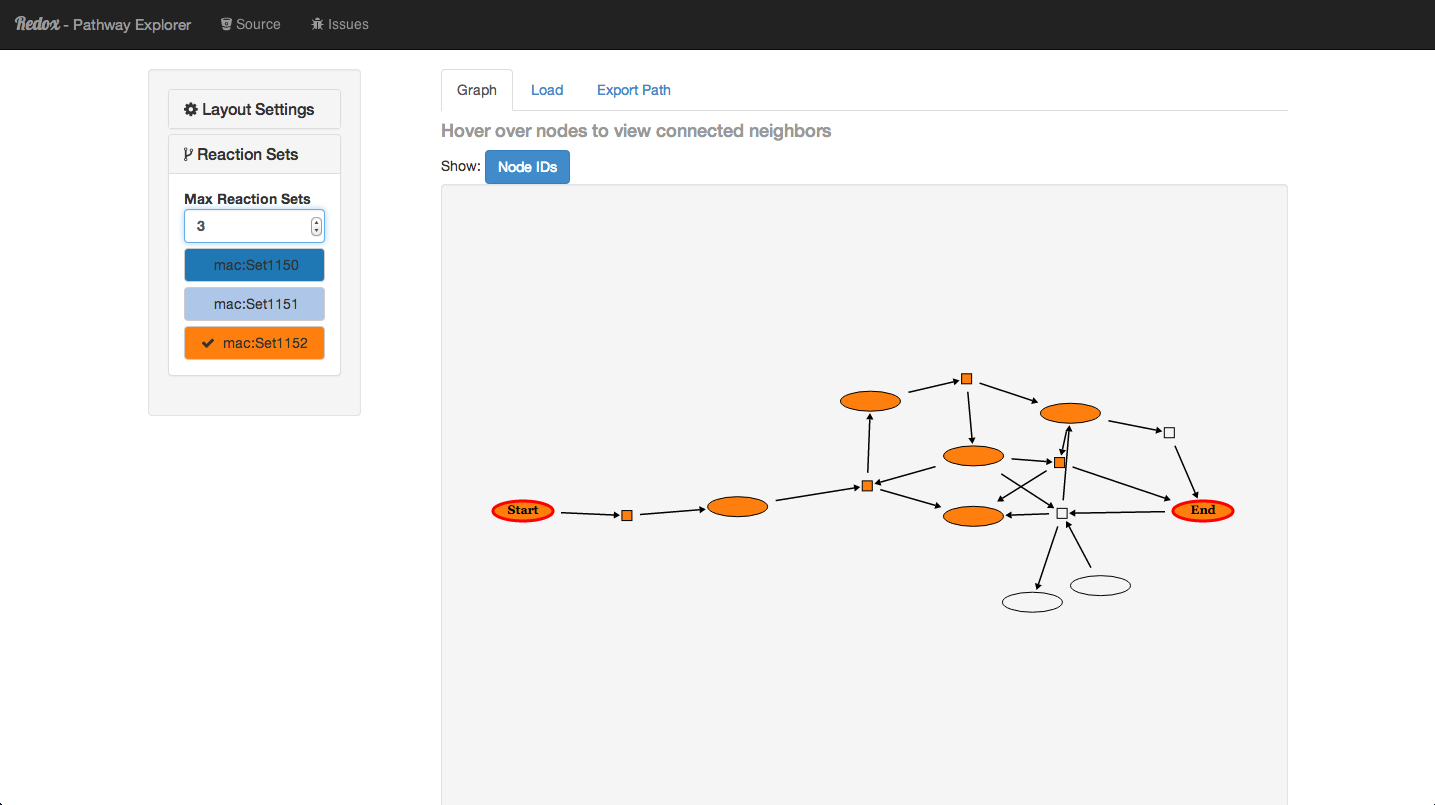
\includegraphics[width=\textwidth,natwidth=610,natheight=642]{images/redox-ui.png}
  \caption{Pathway exploration using Redox}
  \label{Figure:redox}
\end{figure}



\section{Implementation}

\chapter{Carbon: Cloud Workspaces}

\section{Purpose}


\section{Motivation}
\subsection{Reproducibility is crucial for science}
\subsection{Reproducibility is difficult for computational systems biology}
\subsection{Systems biology software is difficult to install}


\section{Solution}
\subsection{Framework for scientific web applications and personal workspaces}
\begin{figure}
  \centering
  \begin{subfigure}[b]{\textwidth}
    \includegraphics[width=\textwidth,page=9,trim=0.37cm 3.65cm 13.1cm 3.3cm, clip=true]{images/Figures.pdf}
    \caption{The Carbon landing page.}
    \label{Figure:carbon-login-landing}
  \end{subfigure}
  \begin{subfigure}[b]{\textwidth}
    \includegraphics[width=\textwidth,page=9,trim=13.1cm 3.65cm 0.37cm 3.3cm, clip=true]{images/Figures.pdf}
    \caption{Once the user is logged in, the navigation bar will populate with available applications.}
    \label{Figure:carbon-login-logged-in}
  \end{subfigure}
  \caption{Carbon provides a user-specific workspaces.}
  \label{Figure:carbon-login}
\end{figure}

\begin{figure}
  \centering
  \begin{subfigure}[b]{\textwidth}
    \includegraphics[width=\textwidth,page=10,trim=0.37cm 3.65cm 13.1cm 3.3cm, clip=true]{images/Figures.pdf}
    \caption{The left sidebar contains a collapsible directory tree view.
      Each directory also contains expandable option buttons for file creation, upload, and deletion.}
    \label{Figure:carbon-workspaces-view}
  \end{subfigure}
  \begin{subfigure}[b]{\textwidth}
    \includegraphics[width=\textwidth,page=10,trim=13.1cm 3.65cm 0.37cm 3.3cm, clip=true]{images/Figures.pdf}
    \caption{New folders can also be created anywhere within the directory tree.}
    \label{Figure:carbon-workspaces-new-folder}
  \end{subfigure}
  \caption{Workspace app is a plugin to Carbon that allows easy file management and browsing of model files.}
  \label{Figure:carbon-workspaces}
\end{figure}

\begin{figure}
  \centering
  \begin{subfigure}[b]{\textwidth}
    \includegraphics[width=\textwidth,page=11,trim=0.37cm 3.65cm 13.1cm 3.3cm, clip=true]{images/Figures.pdf}
    \caption{Users may create new files in the workspace by upload or copy and paste.}
    \label{Figure:carbon-workspaces-file-upload}
  \end{subfigure}
  \begin{subfigure}[b]{\textwidth}
    \includegraphics[width=\textwidth,page=11,trim=13.1cm 3.65cm 0.37cm 3.3cm, clip=true]{images/Figures.pdf}
    \caption{All files can be edited as text, but detected model files also uses Graphene to construct a network layout view.}
    \label{Figure:carbon-workspaces-model-view}
  \end{subfigure}
  \caption{}
  \label{Figure:carbon-workspaces-files}
\end{figure}

\begin{figure}
  \centering
  \begin{subfigure}[b]{\textwidth}
    \includegraphics[width=\textwidth,page=12,trim=0.37cm 3.65cm 13.1cm 3.3cm, clip=true]{images/Figures.pdf}
    \caption{}
    \label{Figure:}
  \end{subfigure}
  \begin{subfigure}[b]{\textwidth}
    \includegraphics[width=\textwidth,page=12,trim=13.1cm 3.65cm 0.37cm 3.3cm, clip=true]{images/Figures.pdf}
    \caption{}
    \label{Figure:}
  \end{subfigure}
  \caption{}
  \label{Figure:}
\end{figure}

\begin{figure}
  \centering
  \begin{subfigure}[b]{\textwidth}
    \includegraphics[width=\textwidth,page=13,trim=0.37cm 3.65cm 13.1cm 3.3cm, clip=true]{images/Figures.pdf}
    \caption{}
    \label{Figure:}
  \end{subfigure}
  \begin{subfigure}[b]{\textwidth}
    \includegraphics[width=\textwidth,page=13,trim=13.1cm 3.65cm 0.37cm 3.3cm, clip=true]{images/Figures.pdf}
    \caption{}
    \label{Figure:}
  \end{subfigure}
  \caption{}
  \label{Figure:}
\end{figure}

\begin{figure}
  \centering
  \includegraphics[width=\textwidth,page=14,trim=0.37cm .65cm 0.37cm 0.3cm, clip=true]{images/Figures.pdf}
  \caption{}
  \label{Figure:}
\end{figure}

\subsection{Python environment for model exploration, analysis, and curation}
\subsection{Convert standard model formats to IPython notebooks}


\section{Implementation}
\subsection{Server Architecture}
\subsubsection{Express.js and Flask}
\subsubsection{MongoDB}
\subsection{Workspace Isolation}
\subsubsection{Linux Containers}
\subsubsection{Services and Ports}
\subsection{Asynchronous Programming}
\subsubsection{Highly Nested Callbacks}
\subsubsection{Use of Promises}
\subsection{Conversion of model formats to IPython notebooks}

\section{Future Directions}
\subsection{Security}

\chapter{Distributed Simulation Servers}
\label{chap:engine}

\section{Purpose}


\section{Motivation}
\subsection{Simulation processes may be are often single threaded and complex models may require long simulation times}
\subsection{Model analysis requires a lot of simulation}
\subsection{The majority of simulation software runs on a single host system}


\section{Solution}
\subsection{Simulation queue}
\subsection{Engine Block}
\subsection{User Interface}


\section{Implementation}
\subsection{Priority queue}
\subsection{Vagrant virtual machines to bootstrap engine blocks}
\subsection{Docker containers for replicating engine cylinders}


\section{Future Directions}

\chapter{Summary}

\section{Scientific Contributions Revisited}

\section{Future Directions}



% bibliography
%
\printbibliography[title=References]
% appendices
%
\appendix
% \include{appendix-graphene-logo}
% \include{appendix-software-availability}

\end{document}
